\documentclass[a4paper,12pt]{article}
%%%%%%%%%%%%%%%%%%%%%%%%%%%%%%%%%%%%%%%%%%%%%%%%%%%%%%%%%%%%%%%%%%%%%%%%%%%%%%%%%%%%%%%%%%%%%%%%%%%%%%%%%%%%%%%%%%%%%%%%%%%%%%%%%%%%%%%%%%%%%%%%%%%%%%%%%%%%%%%%%%%%%%%%%%%%%%%%%%%%%%%%%%%%%%%%%%%%%%%%%%%%%%%%%%%%%%%%%%%%%%%%%%%%%%%%%%%%%%%%%%%%%%%%%%%%
\usepackage{eurosym}
\usepackage{vmargin}
\usepackage{amsmath}
\usepackage{graphics}
\usepackage{epsfig}
\usepackage{enumerate}
\usepackage{multicol}
\usepackage{subfigure}
\usepackage{fancyhdr}
\usepackage{listings}
\usepackage{framed}
\usepackage{graphicx}
\usepackage{amsmath}
\usepackage{chngpage}
%\usepackage{bigints}

\usepackage{vmargin}
% left top textwidth textheight headheight
% headsep footheight footskip
\setmargins{2.0cm}{2.5cm}{16 cm}{22cm}{0.5cm}{0cm}{1cm}{1cm}
\renewcommand{\baselinestretch}{1.3}

\setcounter{MaxMatrixCols}{10}

\begin{document}
\large 
\noindent A general insurance company has sold 5000 Accident Benefit Policies to independent lives.\\\\
\medskip
\noindent The number of claims follows a Poisson distribution with parameter 500. The amount of claim
from individual policy is following a Gamma distribution with parameters $\alpha = 250$ and $\lambda = 0.5$.\\
\medskip

\noindent Calculate the aggregate claim amount paid by the insurer by simulating 5000 values if the
insurer retains only 350 (assume the aggregate claim amount follows a compound Poisson
distribution). 
%%Use seed corresponding to your birth year.

%%%%%%%%%%%%%%%%%%%%%%%%%%%%%%
\subsection*{Solution}


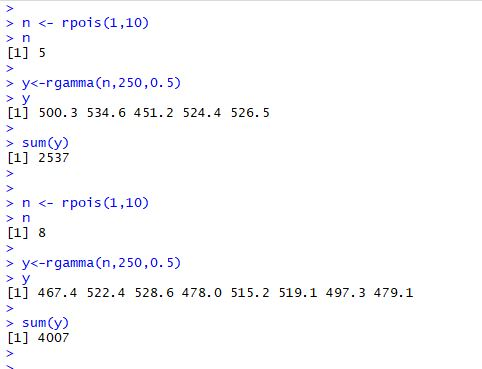
\includegraphics[scale=1.3]{00-B2/images/B2_Agg_Claim_CompoundPoisson.JPG}

\bigskip
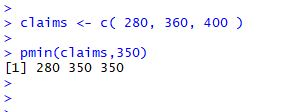
\includegraphics[scale=1.4]{00-B2/images/B2-PairwiseMinimum.JPG}
\newpage 
\begin{framed}
\begin{verbatim}
set.seed(1234)
n <- rpois(5000,500)

Agg_Claim <- rep(0,5000)

for(j in 1:5000){
    y<-rgamma(n[j],250,0.5)
    z<-pmin(y,350)
    Agg_Claim[j] <-sum(z)
    }

\end{verbatim}
\end{framed}

\newpage 

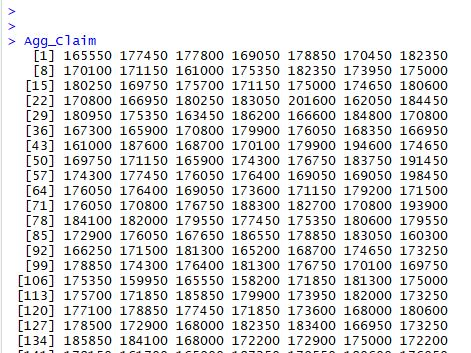
\includegraphics[scale=1.5]{00-B2/images/B2_Agg_Claim_1.JPG}


\medskip
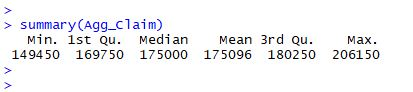
\includegraphics[scale=1.5]{00-B2/images/B2_Agg_Claim_2.JPG}

\newpage 
BLANK
\end{document}
